% intro
For both pixel-based and voxel-based reconstruction, the input data is processed before the actual reconstruction. In our case, this means calibrating the tracking data and handling the different rate of tracking data and ultrasound scans.

% why this is necessary and how it is done
\subsection{Calibration of Tracking Data}

	\begin{figure}[h]
	\centering
	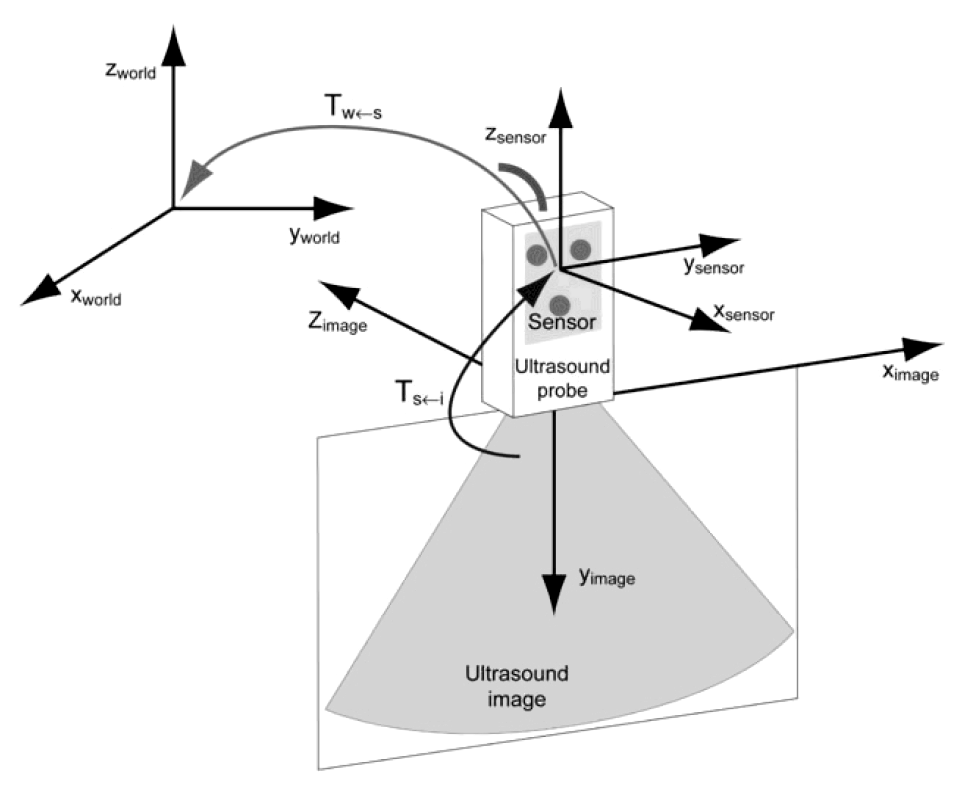
\includegraphics[width=\textwidth]{graphics/tracking_spaces.png}
	\caption[Spaces of a tracking system]{Spaces of a tracking system (used with permission from \cite{mercier2005})}
	\label{fig:tracking_spaces}
	\end{figure}

	Figure \ref{fig:tracking_spaces} shows a tracking system with a sensor attached to an ultrasound probe. The tracking system will give the relation between the sensor and the world space, $T_{w \leftarrow s}$, in the form of a transformation matrix. This transforms coordinates in the space of the sensor to coordinates in the world reference space. However, even though the sensor is tightly attached to the probe, it is not in the origin of the space of the ultrasound images. This relation, $T_{s \leftarrow i}$ varies with each tracking system's setup, so a calibration transformation is required and is part of the input. Before the reconstruction begins this calibration matrix is multiplied into the tracking transformations.

% what this problem is and how it is handled by interpolation
\subsection{Handling Different Tracking and Scanning Rate}

	While the probe catches ultrasound images, the tracking system outputs a series of transformation matrices. Ideally, the tracking system and ultrasound probe should be synchronized such that each b-scan has an associated transformation. However, the tracking system used in this thesis has a slighter higher rate than the probe.  Is is assumed that both systems start and stop at the same time. As an example, one of the input set used in this thesis has 434 b-scans and 520 tracked positions.
	
	This is handled by interpolating the tracking data stream between the b-scan stream. Since the tracking data consists of $4 \times 3$ matrices of floating point values, it is obviously easier to interpolate than the b-scans with thousands of pixels. Each b-scan and tracked position has an associated timetag, but the probe and tracking system use clocks with different timestamp resolutions.
	
	Given these considerations, the timetags are first normalized to the same unit by first subtracting the first timetag from all timetags in each stream respectively. In this manner, each stream begins with the time 0. Then, each tracking timetag is multiplied by the ratio between the last b-scan timetag and the last tracking timetag. This makes the tracking timetags end with the same timetag as the b-scan timetags.
	
	\begin{figure}[h]
	\centering
	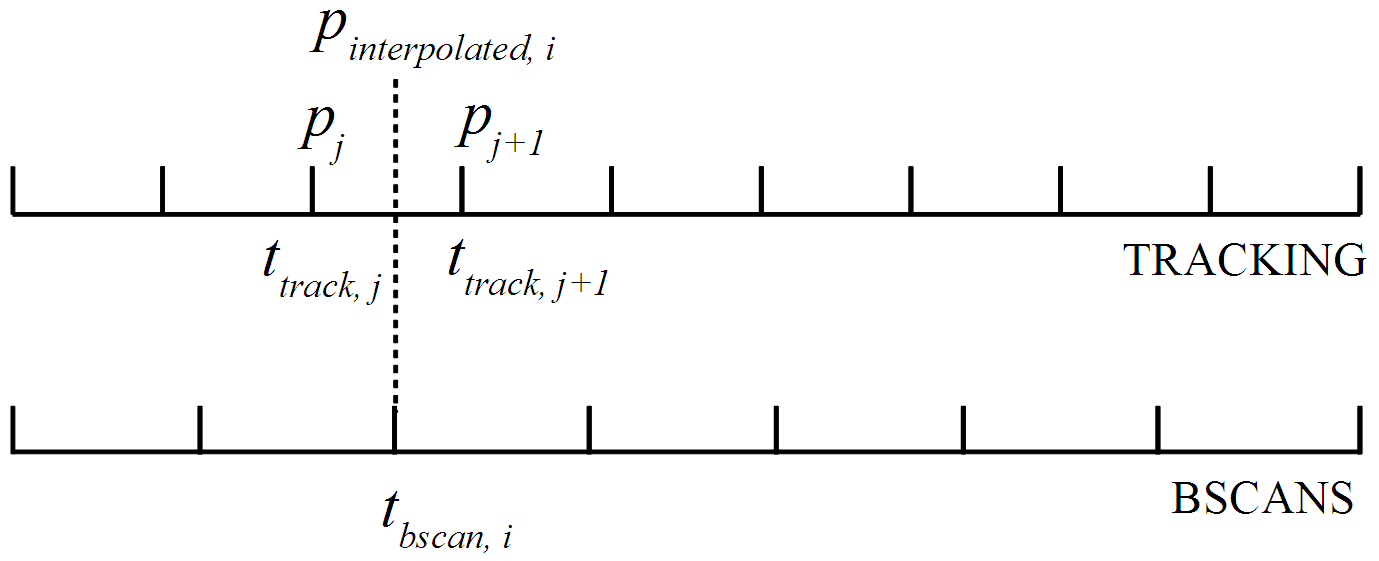
\includegraphics[width=\textwidth]{graphics/tracking_scanning_interpolation.png}
	\caption{Interpolation of tracking data after timetag normalization}
	\label{fig:tracking_scanning_interpolation}
	\end{figure}
	
	 Figure \ref{fig:tracking_scanning_interpolation} shows how the tracking data is interpolated using the normalized timetags. Each interpolated value is given by Equation \ref{eq:tracking_scanning_interpolation} where $p_{interpolated,i}$ is the value interpolated between $p_j$ and $p_{j+1}$ given the timetags $t_{bscan}$ and $t_{track}$ of the b-scans and tracking data. The values in the first and last tracking matrices need not be interpolated (because of tracking and scanning starting and stopping at the same time).
	 
	\begin{equation}
		p_{interpolated,i} = p_j + \frac{t_{bscan,i} - t_{track,j}}{t_{track,j+1} - t_{track,j}} \cdot (p_{j+1} - p_{j})
	\label{eq:tracking_scanning_interpolation}
	\end{equation}